% DOCUMENT FORMATING
\documentclass[12pt]{article}
\usepackage[margin=1in]{geometry}

% PACKAGES
\usepackage{amsmath} % For extended formatting
\usepackage{amssymb} % For math symbols
\usepackage{amsthm} % For proof environment
\usepackage{array} % For tables
\usepackage{enumerate} % For lists
\usepackage{extramarks} % For headers and footers
\usepackage{fancyhdr} % For custom headers
\usepackage{graphicx} % For inserting images
\usepackage{multicol} % For multiple columns
\usepackage{verbatim} % For displaying code
\usepackage{tkz-euclide}
\usepackage{pgfplots}
\usepackage{mathtools}


% SET UP HEADER AND FOOTER
\pagestyle{fancy}
\lhead{\MyCourse} % Top left header
%\chead{\MyTopicTitle} % Top center header
\rhead{\MyAssignment} % Top right header
%\lfoot{\MyCampus} % Bottom left footer
\cfoot{} % Bottom center footer
%\rfoot{\MySemester} % Bottom right footer
\renewcommand\headrulewidth{0.4pt} % Size of the header rule
\renewcommand\footrulewidth{0.4pt} % Size of the footer rule




% ----------
% TITLES AND NAMES 
% ----------

\newcommand{\MyCourse}{Math 241}
\newcommand{\MyAssignment}{Worksheet 2}
%\newcommand{\MySemester}{Spring 2020}
%\newcommand{\MyCampus}{University of Hawaii at Manoa}

% ----------
% BEGIN DOCUMENT
% ----------

\begin{document} 
\begin{enumerate}
    \item Decompose the following functions $F(x)$ into three simpler functions $f,g,h$ so that $F(x) = (f\circ g\circ h)(x)$. Do not use the identity/trivial function for $f,g$ or $h$.
    \begin{enumerate}
        \item $F(x) = \sqrt{x^2+4}$
        \vfill
        \item $F(x) = \sin^2(2x+1)$
        \vfill
        \item $F(x) = \tan(\cos(x^3))$
        \vfill
    
    \end{enumerate}
\pagebreak
    
    \item The graph of $f(x)$ is drawn below. Find the following values and limits if they exist. If the limit is $+\infty$ or $-\infty$ specify which  instead of ``does not exist."

    \begin{center}
        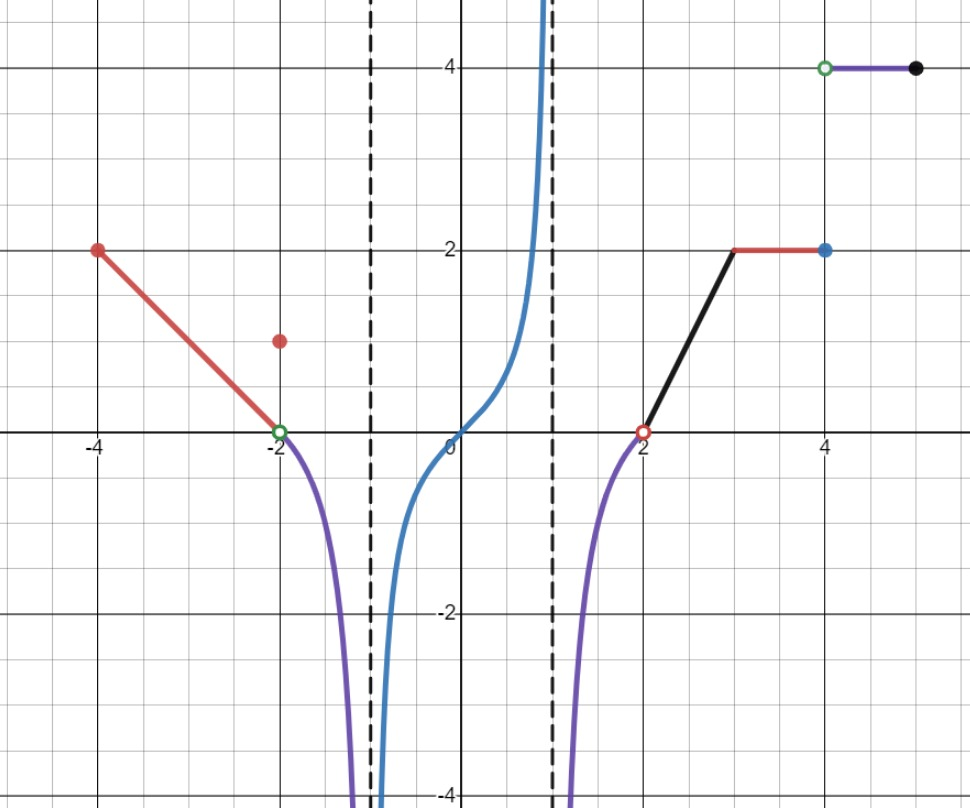
\includegraphics[width=0.75\textwidth]{Images/WS2pic2.jpeg}
    \end{center}

    \begin{enumerate}
        \begin{multicols}{2}
        \item $\displaystyle\lim_{x\to -2^-} f(x)$
        \item[]
        \item $\displaystyle\lim_{x\to -2^+} f(x)$
        \item[]
        \item $\displaystyle\lim_{x\to -2} f(x)$
        \item[]
        \item $f(-2)$
        \item[]
        \item $\displaystyle\lim_{x\to -1^-} f(x)$
        \item[]
        \item $\displaystyle\lim_{x\to -1^+} f(x)$
        \item[]
        \item $\displaystyle\lim_{x\to -1} f(x)$
        \item[]
        \item $\displaystyle\lim_{x\to 1^-} f(x)$
        \item[]
        \item $\displaystyle\lim_{x\to 1^+} f(x)$
        \item[]
        \item $\displaystyle\lim_{x\to 2^-} f(x)$
        \item[]
        \item $\displaystyle\lim_{x\to 2^+} f(x)$
        \item[]
        \item $\displaystyle\lim_{x\to 2} f(x)$
        \item[]
        \item $f(2)$
        \item[]
        \item $\displaystyle\lim_{x\to 4^-} f(x)$
        \item[]
        \item $\displaystyle\lim_{x\to 4^+} f(x)$
        \item[]
        \item $f(4)$
        \item[]
        \end{multicols}
    \end{enumerate}

    \pagebreak

    \item Using the rules for limits, compute the following limits. If the limit is $\pm \infty$ state which. If the limit does not exist, write DNE. \emph{Don't forget to keep the limit notation until you take the limit!}

    \begin{enumerate}
        \item $\displaystyle\lim_{x\to 3} \dfrac{x^2-4x+3}{x^2-9}$
        \vfill
        \item $\displaystyle\lim_{x\to 2} \dfrac{x^2+3x-2}{x-1}.$
        \vfill
\pagebreak
        
        \item $\displaystyle\lim_{x\to 2^+} \dfrac{x^2-2x-8}{x^2-4x+4}$
        \vfill 
        \item $\displaystyle\lim_{x\to 0} \dfrac{x^2-x}{x(x+2)}$
        \vfill
    \end{enumerate}
\end{enumerate}
\end{document}